%\documentclass[11pt, oneside]{article}   	
%\usepackage{geometry}    
%\geometry{letterpaper}                 		
\input preamble.tex
\newcommand{\ig}[2][width=4in]{\includegraphics[#1]{#2}}    		
\usepackage{graphicx}					
\usepackage{amssymb}
\usepackage{pgfplotstable}
\usepackage{float}
\usepackage{caption}
\captionsetup[table]{justification=justified,singlelinecheck=false, position=bottom}
\begin{document}

\header {\today}							
\title{Rutherford Scattering}
\author{Ekta Patel \& Brandon Booth-Dunbar}

\section{Abstract}
\begin{em} In this lab, we verify the Rutherford formula for nuclear scattering in 1909. Their experiment led to the confirmation of the existence of an atomic nucleus, thus destroying the plum pudding model  developed by J. J. Thomson. Rutherford's team successfully disproved Thomson's model by observing a significant amount of charged alpha particles scattering back from a thin sheet of gold foil rather than passing through it with only a few deflections. Therefore, they were able to confirm that an atom consists of a dense nucleus surrounded by a less dense cloud of electrons surrounding the heavy nucleus, instead of an even distribution of mass throughout the atom. The distribution of alpha particles scattered by gold foil can be observed as a function of the scattering angle, which relies on the distance between the foil and the gold source. \end {em}

\section{Theory}
%B&E
Geiger and Marsden formed the first preliminary theory for the Rutherford model of the atom. They were able to gather that most $\alpha$-particles, He nuclei, passed right through a thin foil without being deflected. However, there were many particles that experienced large angle scattering. The differential scattering cross section will be determined in this lab: 
\begin{equation} \frac{d\sigma}{d\Omega}(\theta)\Delta\Omega=\frac{number\;of\; particles\; per\; unit\; time\;into\;a \;solid\; angle\; \Delta\Omega(\theta)}{(number \;of\; scatterers)\times (incident\; flux)} \end{equation}

Based on the previous definition, Rutherford was able to show that a positively charged nucleus has a differential scattering cross-section for charged particles that is given by:
\begin {equation}\label{scattering} \frac{d\sigma}{d\Omega}(\theta)= \frac{Z^2z^2e^4}{16E^2} \frac{1}{sin^4(\theta/2)}\end{equation} where $Ze$ is nuclear charge, $ze$ is charge of the scattered particle and $E$ is the energy of the scattered particle. $\theta$ is the scattering angle. However, we can see that this equation does not give appropriate units for a number of particles per area, instead we have $\frac{C^4}{J^2}$.
In order to correct this dimensional analysis disagreement, we look at the kinetic energy of the alpha particle, $E$, which is:
\begin{equation} E=\frac{1}{2}mv^2.\end{equation} However, when colliding alpha particles head on with the nucleus, all of the kinetic energy is turned into potential energy and the particle is at rest, so $E$ is also:
\begin{equation} E=\frac{q_1q_2}{4\pi\epsilon_0 b}.\end{equation} In the previous equation, $q_1=Ze$ and $q_2=ze$. We can solve for $b$, the distance between the center of the alpha particle and the center of the nucleus, where\begin{equation} b= \frac{Zze^2}{2\pi \epsilon_0 mv^2}.\end{equation}
Therefore, Equation \ref{scattering} can be rewritten as\begin{equation}\frac{d\sigma}{d\Omega}(\theta)=\left(\frac{1}{4b}\right)^2\frac{1}{sin^4(\theta/2)}.\end{equation}
\newline The scattering cross section can then be used to find the rate of detected particles, $N_2$, which is expressed in\ terms of $N_0$, the total number of particles emitted by the source per unit solid angle. Using the geometry of the set up and the Rutherford formula, the rate of detected particles is determined by the following formula
\begin{equation} N_2=n\frac{d\sigma}{d\Omega}(\theta)\Delta\Omega_2\times (incident\;flux)\end{equation} where $n$ is the number of scattering centers. The incident flux is given by $\frac{N_0}{R_1^2}$, which correspond to the figures in the next section. Then, $N_2$ is:
\begin{equation} N_2=\frac{nN_0}{R_1^2}\frac{d\sigma}{d\Omega}\Delta\Omega_2.\end{equation}
The scattering angle, $\theta$, varies with the changing distance $Y$ in the apparatus. Using the geometry of the setup, this formula can be given as
\begin{equation} \label{complicated}N_2=N_0\times \left( \frac{nA_2Z^2z^2e^4}{R_1^2r_1^2 16 E^2}\right)\times \left(\frac{cos\theta_2 sin\theta_2^2}{sin(\theta/2)^4}\right) \end {equation}\\or more simply as\begin{equation}  \label{simple}N_2=N_0\times G\times f(Y). \end{equation} Here G is the atomic factor that accounts for the force between the gold atoms and the scattered alpha particles as they pass through the gold foil. Here, we take for granted that the solid angles we mention are averages and that the scattering center is an average scattering center since we do not know where on the surface area of the gold foil each, or most, of the alpha particles will pass through. 
\section{Experimental Methods}
\subsection{Apparatus}
\begin{figure}[H]
\begin{center}
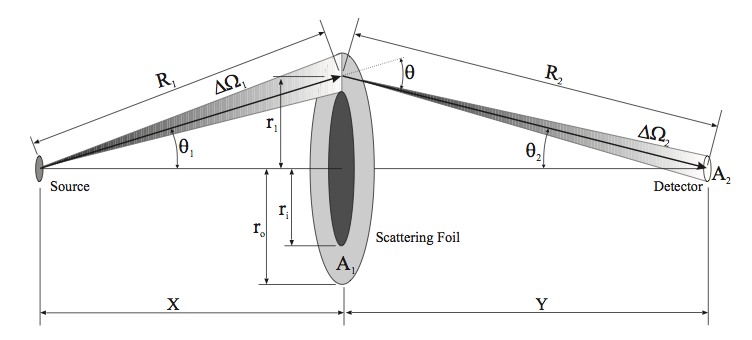
\includegraphics[width=7in]{apparatus.png}
\caption{Experimental geometry.}
\end{center}
\end{figure}
\subsection{Procedures}
\subsection{Calibration}
\subsection{Recording Data}

\section{Results and Discussion}
\subsection{The Scattering Angle Distribution}
Using Equations \ref{simple} and \ref{complicated}, solving the equation for $f(Y)$ gives the angular distribution as a function of Y. We can plot $Y$ vs. $f(Y)$ for a range of 0 cm to 20 cm to get a curve that we can use to fit our experimental results. We solve for f(Y) in the following steps:
\begin{equation} f(Y)=\frac{cos\theta_2 sin\theta_2^2}{sin(\theta/2)^4} \end{equation} where
\begin{equation} \theta_1=tan^{-1}\left(\frac{r_1}{X}\right)\end{equation} and
\begin{equation} \theta_2=tan^{-1}\left(\frac{r_1}{Y}\right)\end{equation} and
\begin{equation} cos\theta_2=\frac{Y}{\sqrt{Y^2+r_1^2}} \end{equation} and
\begin{equation} sin\theta_2^2=\frac{r_1^2}{Y^2+r_1^2}, \end{equation} therefore:
\begin{equation} f(Y)= \frac{\frac{Y}{\sqrt{Y^2+r_1^2}} \frac{r_1^2}{Y^2+r_1^2}}{sin(0.5(tan^{-1}\left(\frac{r_1}{X}\right) + tan^{-1}\left(\frac{r_1}{Y}))\right)^4.} \end{equation}\\
We know the following quantities as they are given in the lab manual because we cannot open the apparatus and check them for ourselves:
\begin{table}[H]
\begin{center}
\begin{tabular}{|c|c|}\hline
Quantity & Description \\ \hline 
$r_s=0.32\pm0.01cm$ & radius of source\\ \hline 
$X=7.22\pm0.01cm$ & source to plane of scattering foil\\ \hline
$r_i=2.30cm$ & radius of the inside of the scattering foil\\ \hline
$r_o=2.70cm$ & radius of the outside of the scattering foil\\ \hline
$r_d=0.48cm$ & radius of the detector\\ \hline
\end{tabular}
\caption{Several components of the apparatus that have been measured for us so that we do not have to disassemble the radioactive source.}
\end{center}
\end{table}
Plotting this function for f(Y) over an interval of 0 to 20cm, we have:
\begin{figure}[h!]
\begin{center}
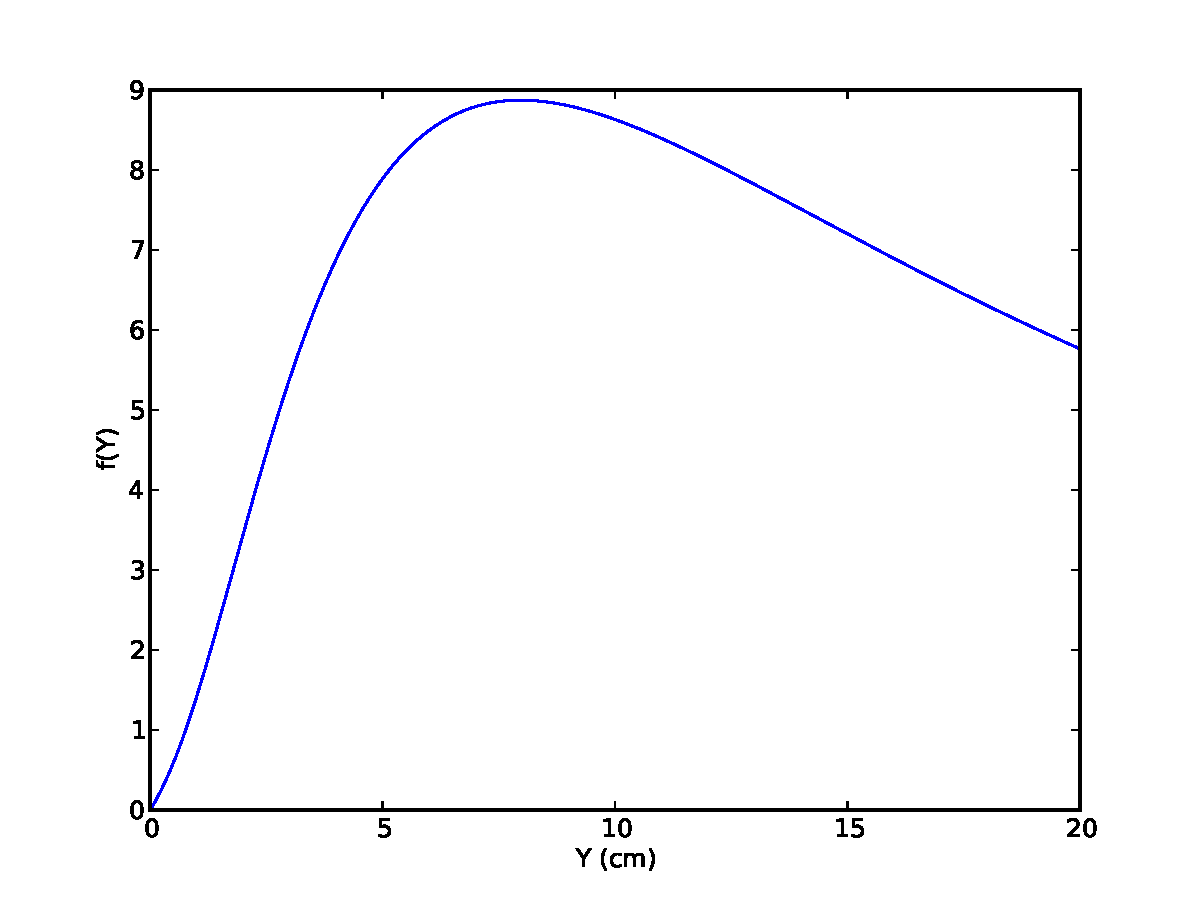
\includegraphics[width=4in]{preliminary_plot.pdf}
\caption{The angular distribution for the third term in the rate of detected particles($N_2$) that varies with the scattering angle as a function of length. The peak occurs in the vicinity of 8 cm.}
\end{center}
\end{figure}

\subsection{Determining $G$ \& $N_0$}
%EKTA FINISH THIS SECTION
Figure 3 below shows our preliminary data set taken over a range from 3cm to 18cm in 1cm intervals. At each value for Y, the distance from the gold foil to the source, we counted for 20 minutes. Our data shows a peak around 10cm as opposed to the 8cm prediction given in the angular distribution plot above. It can be seen however, that the peak distance is relative to where on the apparatus one begins to record data. The axis on which we can move the source in an out of the apparatus chamber was measured to be 19.7cm$\pm$.01cm long. The length along this axis at which we choose to begin measurements however, is dependent on our gains for the linear amplifier in the electronic schematic of the apparatus, and therefore arbitrary to the length at which we make our zero reference point. Since we are able to tune our discriminator so that about 20\% of the alpha particles are rejected, our data is simply shifted along the $Y$ parameter by about 3 centimeters in the positive direction. 
\begin{figure}[H]
\begin{center}
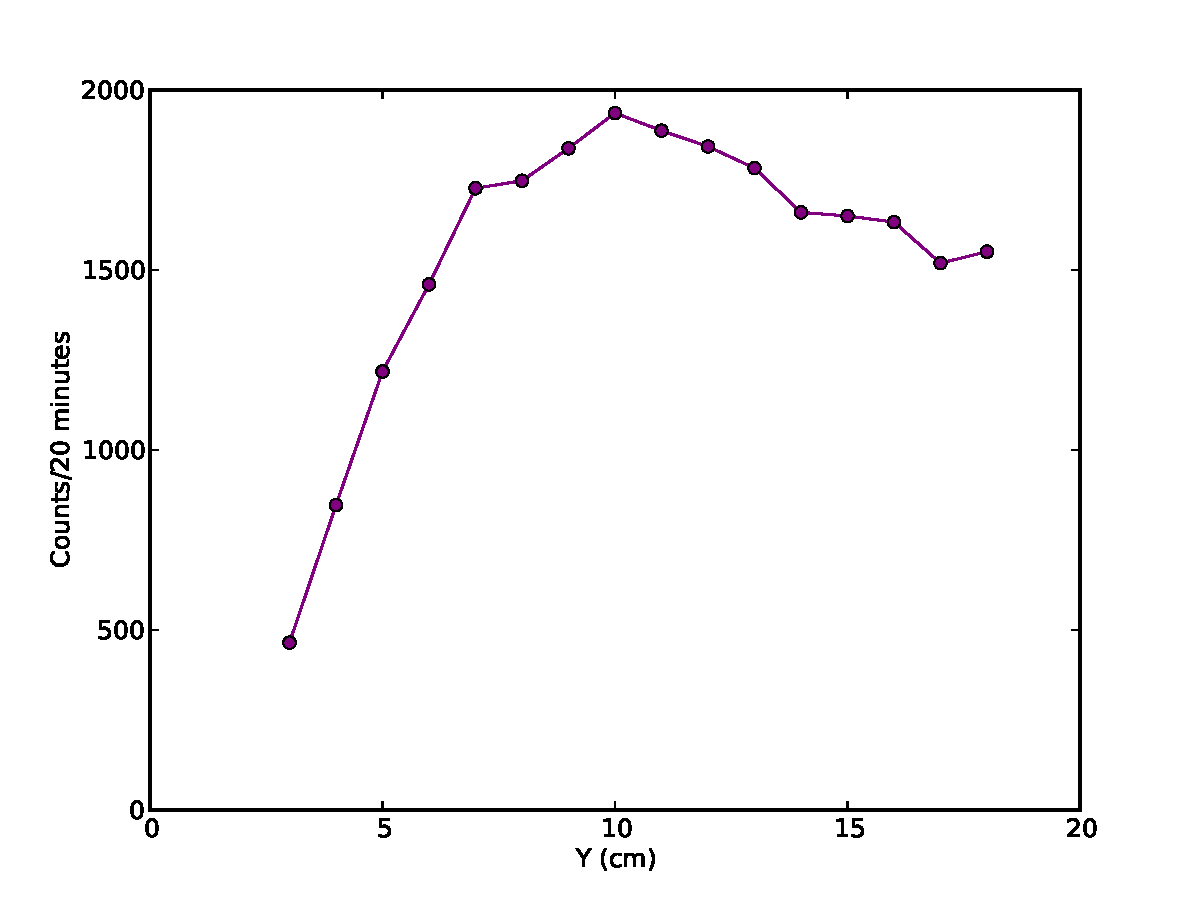
\includegraphics[width=4in]{firstrun.pdf}
\caption{The first run of data taken from 3cm to 18cm in intervals of 1cm.}
\end{center}
\end{figure}
After seeing a curve that represented the same shape as that of $f(Y)$, we went back and collected data in between the intervals we previously recorded so that we could have a full set of data from 3cm to 18cm in 0.5cm steps. 
\begin{figure}[H]
\begin{center}
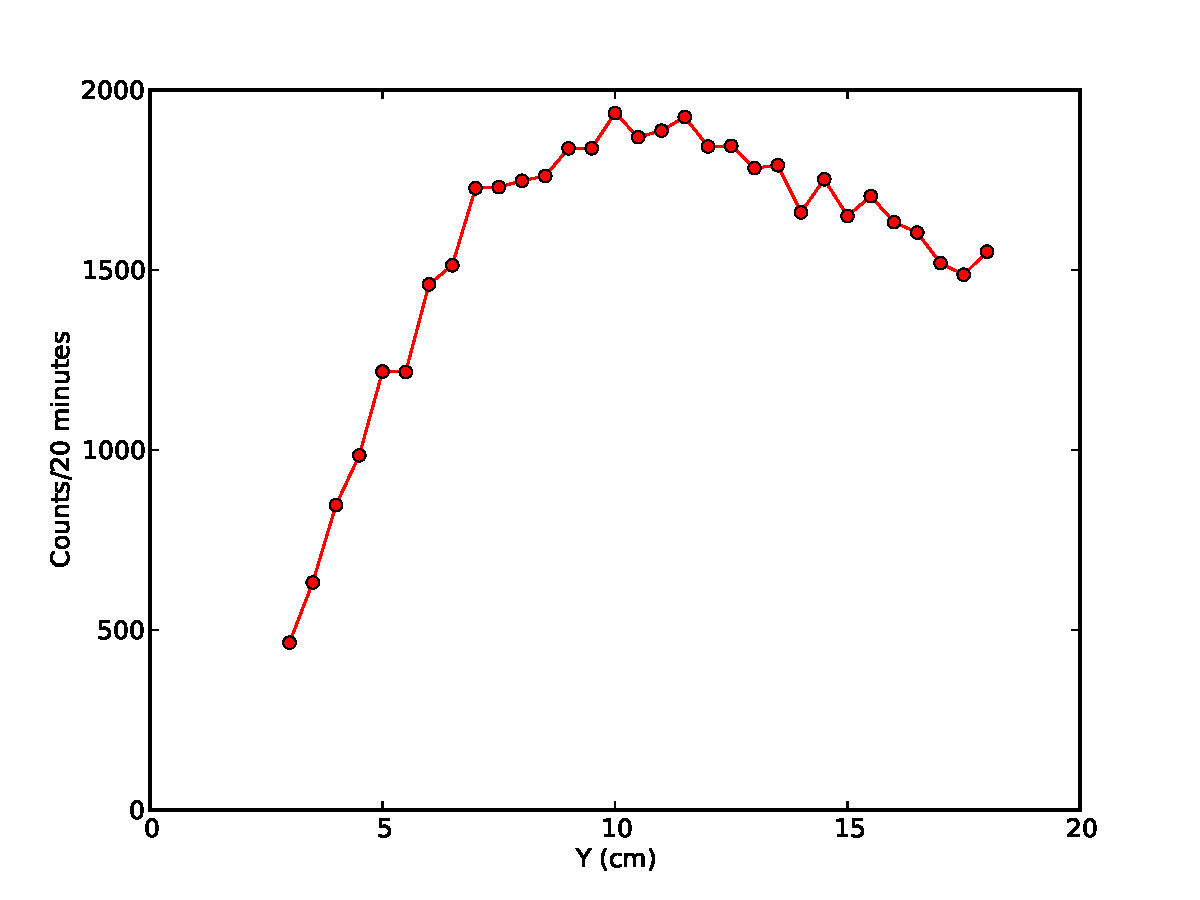
\includegraphics[width=4in]{secondrun.pdf}
\caption{The first run of data taken from 3cm to 18cm in intervals of 1cm combined  with an additional run with points taken in intervals of 0.5cm to obtain more statistics.}
\end{center}
\end{figure}

Since we cannot find a value for $N_0$ directly because it would require dissembling the apparatus chamber and placing the detector directly next to the source, we can indirectly calculated it using the three values that we know or have measured, $G$, $N_2$, and $f(Y)$. First, G is simple a factor that is a result of combination of known values in this apparatus. 
\begin{equation}G=\frac{nA_2Z^2z^2e^4k^2}{R_1^2r_1^2  E^2}\end{equation}
That factors that are included in $G$ are listed below:

\begin{table}[H]
\begin{center}
\begin{tabular}{|c|c|c|}\hline
Quantity & Description & Value\\ \hline
 $n=\left(\frac{\rho N_A}{A_g}\right)A_1 t$ & Total number of scattering centers& $1.491\times10^{19}$ \\ \hline
 $\rho$ & Density of Gold &$1.93\times10^4 kg/m^3$ \\ \hline
$N_A$ & Avogadro's Number &  $6.022\times10^{23}$\\ \hline
$A_g$ & Atomic weight of Gold & $196.97 u= 0.197 kg/mol$ \\ \hline
$A_1=\pi r_o^2-\pi r_i^2 $ & Area of scatting foil& $1.257\times10^{-4} m^2$ \\ \hline
 $t$ & Thickness of scattering foil & $2\times10^{-6} m$\\ \hline
$A_2=\pi r_d^2$ & Area of the detector & $1.508\times10^{-4}m^2$\\ \hline
$Ze$ & Nuclear charge &$79\times (1.6\times^10^{-19} C)$\\ \hline
$ze$ & Alpha particle charge & $2\times(1.6\times^10^{-19} C)$\\ \hline
$E$ & Energy of scattered particle &$4.4MeV=7.0496\times10^{-13}J$\\ \hline
$R_1$ & Hypotenuse from source to scattering foil& $0.03118m$\\ \hline
$r_1$ & Average scattering center & $0.025 m$ \\ \hline
$k$ & Coulomb's constant & $9\times10^9 N\cdot m/ C^2$\\ \hline

\end{tabular}
\caption{All values needed to calculate the factor G as given by the lab manual and the period table.}
\end{center}
\end{table}
Therefore, $G=8.932\times10^{-6}$. We cannot propagate error on the value for $G$ because the values that we are using are taken for granted since we cannot make our measurements of the apparatus that are inside the chamber. We can now use the calculated value for $G$, the angular distribution $f(Y)$ and the experimentally collected count rates, $N_2$ to determine $N_0$. 
%%%%% error propagation, what do our results mean, anything else i forgot?

\begin{figure}[H]
\begin{center}
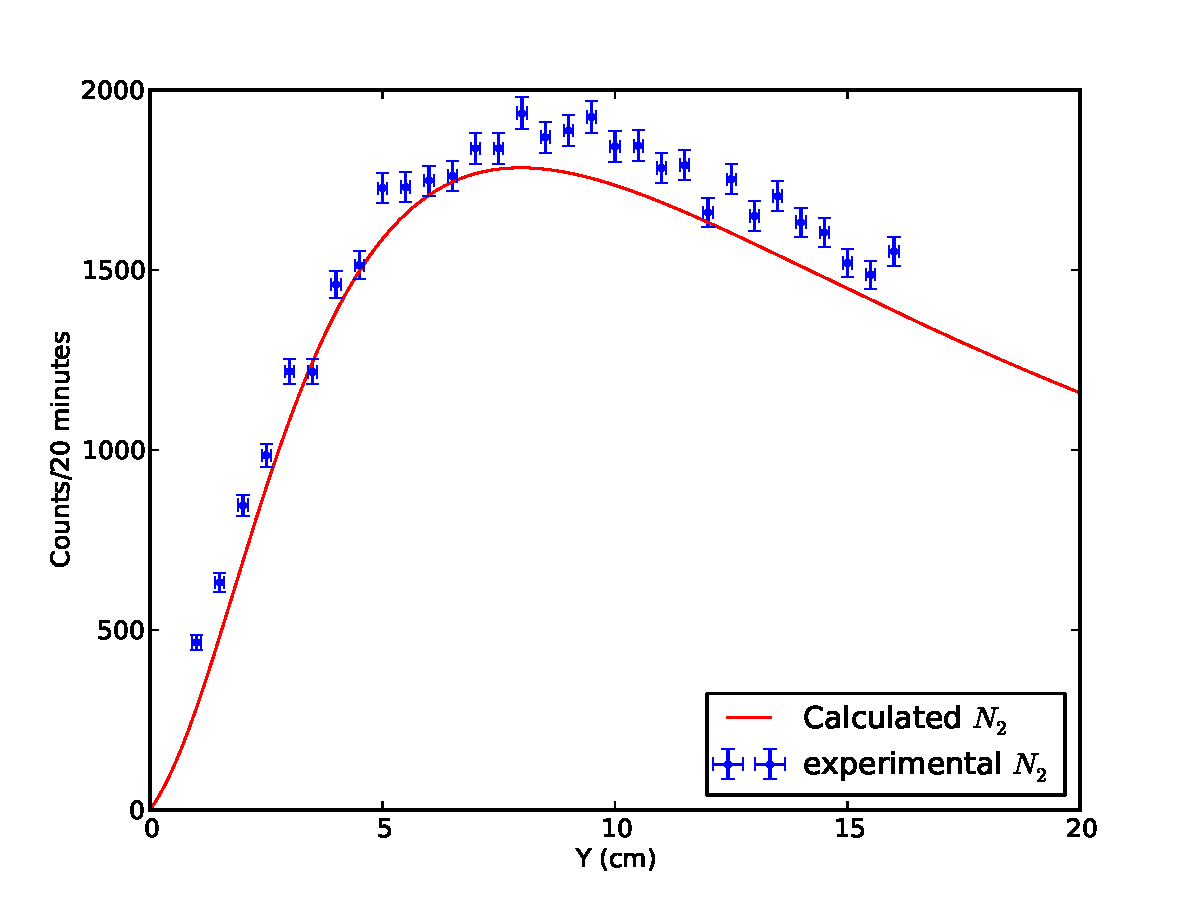
\includegraphics[width=5in]{N2.pdf}
\caption{The calculated value for $N_2$ is shown in red, while our experimental value for $N_2$ is given in the blue data points with error bars corresponding to $\sqrt{\#\; of\; counts}$ per data point.}
\end{center}
\end{figure}

\subsection{Finding the Atomic Number ($Z$)}
The atomic number of gold, given by $Z$, cannot be found using our data because we would need to disassemble the apparatus and place the source right next to the detector in order to determine the proper value for $N_0$. $Z$ is a factor in $G$, so when we rearrange Equation \ref{simple} appropriately, we have: 
\begin{equation}G(Z)= \frac{N_2}{N_0 \times f(Y)}. \end {equation} 
In the above equation, we have values for $N_2$ and a distribution to represent $f(Y)$, but if we cannot experimentally determine $N_0$,  we do not have enough known variables to solve for $Z$. Therefore, we accept that the atomic number of Gold is 79 as given by the periodic table. 
\subsection{Calculating the Nuclear Radius Upper Limit}
The upper limit of the nucleus radius can be determined from the impact parameter, $b$, which we derived earlier in section 2. It is the distance from the center of the alpha particle to the center of the nucleus. The alpha particles do not have enough force to penetrate the nucleus a significant amount compared to the radius of the nucleus, so even though $b$ is the sum of the alpha particle radius and the nucleus radius, we can assume that it is a good approximation for the upper limit of the nuclear radius. Therefore, we know that $b$ is: \begin{equation} \label{b}b= \frac{Zze^2}{2\pi \epsilon_0 mv^2}.\end{equation} Here, we are also making the assumption that the alpha particles hits the nucleus head on and deflects back along a straight line 180$^\circ$ from its initial impact. The quantities in Equation \ref{b} are:
\begin{itemize}
\item $Ze=79\times (1.6\times^10^{-19} C)$
\item $ze= 2\times(1.6\times^10^{-19} C)$
\item $\frac{1}{4\pi\epsilon_0}=9\times10^9 N\cdot m/ C^2$
\item $m=6.7\times10^{-27} kg$
\item $v=2\times 10^7 m/s$
\end{itemize}
Therefore, \begin{equation} b= \frac{(79\times (1.6\times^10^{-19} C))(2\times(1.6\times^10^{-19} C))(9\times10^9 N\cdot m/ C^2)}{(6.7\times10^{-27} kg)(2\times 10^7 m/s)^2}=2.7\times10^{-14}m.\end{equation}
The upper limit on the nuclear radius of Gold is $2.7\times10^{-14}$m as calculated from the parameters given the setup that we have for this experiment.


\section{Conclusion}
%Brandon


\begin{thebibliography}{99}
\bibitem{electron}Sleator, Tycho, and Windt, David, \begin{em}Rutherford Scattering. \end{em}Experimental Physics. V85.0112. Spring, 2011.
\end{thebibliography}

\section{Appendix}
\begin{table}[H]
\begin{tabular}{|c|c|}\hline
Y (cm) & Counts/ 20 min\\ \hline
3.0 & 465  \\ \hline
4.0 &  847 \\ \hline
5.0 &  1218 \\ \hline
6.0 &  1460 \\ \hline
7.0 &  1727\\ \hline
8.0 &  1748 \\ \hline
9.0 &  1838\\ \hline
10.0 &  1936\\ \hline
11.0 &  1867\\ \hline
12.0 &  1843\\ \hline
13.0 &  1783\\ \hline
14.0 &  1660\\ \hline
15.0 &  1650\\ \hline
16.0 & 1633 \\ \hline
17.0 &  1519\\ \hline
18.0 &  1551\\ \hline
\end {tabular}
\caption{First run of data taken from 3cm to 18cm in intervals of 1cm.}
\end{table}

\begin{table}[H]
\begin{tabular}{|c|c|}\hline
Y (cm) & Counts/ 20 min\\ \hline
3.5 & 632 \\ \hline
4.5 &  985 \\ \hline
5.5 &  1217 \\ \hline
6.5 &  1513 \\ \hline
7.5 &  1730\\ \hline
8.5 &  1741 \\ \hline
9.5 &  1838\\ \hline
10.5 &  1869\\ \hline
11.5 &  1925\\ \hline
12.5 &  1845\\ \hline
13.5 &  1791\\ \hline
14.5 &  1752\\ \hline
15.5 &  1705\\ \hline
16.5 & 1604\\ \hline
17.5 &  1487\\ \hline
\end{tabular}
\caption{Second run of data taken from 3.5 cm to 17.5cm in intervals of 1cm.}
\end{table}

\end{document}


